\subsection{a}
Assuming the container is a cone, its volume V(t) is \begin{equation} \label{eq:V}
    V(t) = \frac{h(t) \cdot {r(t)}^2 \pi}{3} = \frac{ \tan\left( \frac{\pi}{2} - \theta \right) \pi}{3}{h(t)}^3 
\end{equation}

\subsection{b}
\begin{equation}
\begin{split}
    &h(\tau) = 0 \\
    \implies &h_0^{\frac{5}{2}} = \frac{ 5a^2 \sqrt{2g} }{ 2\tan^2\left(\frac{\pi}{2} - \theta\right) } \tau \\
    \therefore \ &\tau = h_0^{\frac{5}{2}} \frac{ 2\tan^2\left(\frac{\pi}{2} - \theta\right) }{ 5a^2 \sqrt{2g} }\\
\end{split}
\label{eq:tau}
\end{equation}
Assuming $\theta = \frac{\pi}{4}; \ g=\SI{9.8}{\meter\per\second\squared}$ and replacing the given values:
\begin{equation}
    \tau = {(0.30)}^{\frac{5}{2}} \frac{2 \tan^2\left(\frac{\pi}{2} - \frac{\pi}{4} \right)}{ 5{(0.01)}^2 \sqrt{2\cdot 9.8} }
    = \SI{44.5}{\second}
\end{equation}
\begin{figure}[h]
	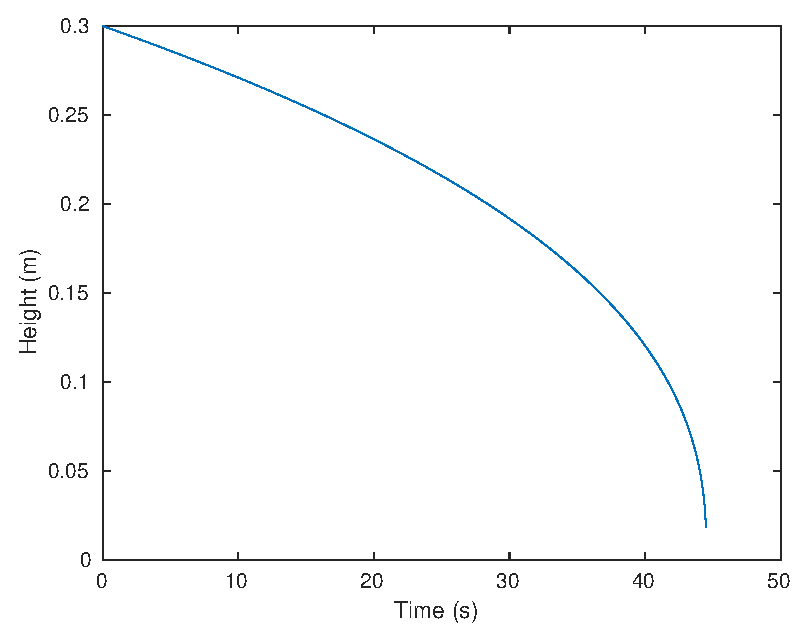
\includegraphics[scale=0.65, center]{./eps/topic5_b.eps}
	\caption{Height variation from $t$ = 0 to $t=\tau=44.5$ }
	\label{fig:Topic5-b}
\end{figure}
As can be seen in Figure \ref{fig:Topic5-b}, the minimum height is \SI{5}{\centi\meter}, which makes the equation not particularly valid -- especially considering we start with a height of \SI{30}{\centi\meter}.
Changing the angle heavily affects how close we are able to get to a height of zero, but this will be discussed subsequent questions.
\lstinputlisting[caption={Topic 5. Question b}]{"./files/topic5/b.m"}

\subsection{c}

Unsurprisingly, the closer to $\frac{\pi}{2}$, the less time it takes to empty the container.
This means that we are approaching the shape of a cylinder, rather than a cone.
Physically this requires a widening of the outlet, decreasing the speed of the liquid coming out.
Furthermore, this points out an interesting feature of graph -- at smaller angles the difference between both heights is far bigger than at larger angles.   

\pagebreak

\begin{figure}[]
	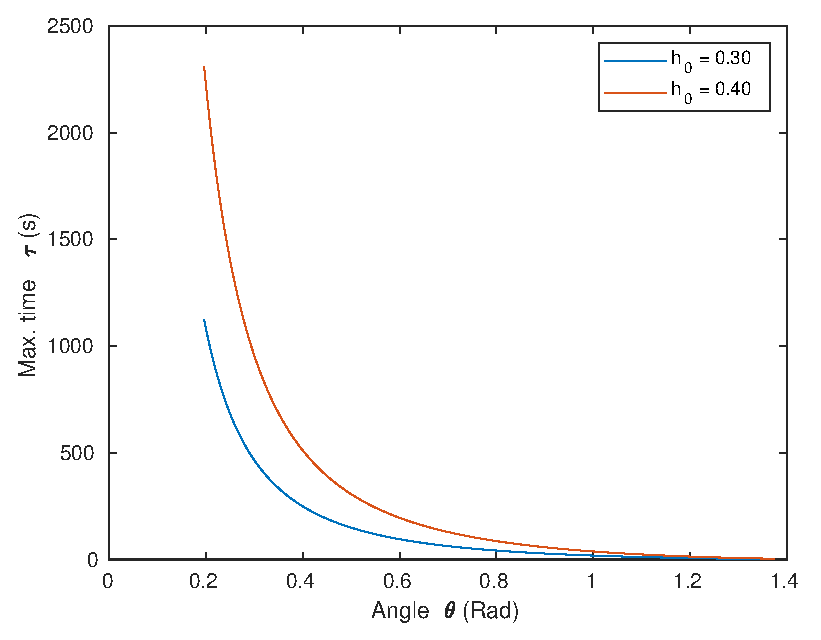
\includegraphics[scale=0.65, center]{./eps/topic5_c.eps}
	\caption{Variation of maximum time $\tau$ with the angle}
	\label{fig:Topic5-c}
\end{figure}

\lstinputlisting[caption={Topic 5. Question c}]{"./files/topic5/c.m"}

\subsection{d}
Rearranging Equation (\ref{eq:tau}) and replacing it into the given expression:
\begin{equation*}
    \frac{ 5a^2 \sqrt{2g} }{ 2\tan^2\left(\frac{\pi}{2} - \theta\right)} = \frac{h_0^{\frac{5}{2}}}{\tau}
\end{equation*}
\begin{equation}
\begin{split}
    &h(t) = {\left[
        h_0^{\frac{5}{2}} - t \cdot \frac{
            h_0^{ \frac{5}{2} }
            }{\tau}    
            \right]}^\frac{2}{5} \\
    \implies &\dot{h}(t) = \frac{d}{dt}h(t) =\frac{2}{5} {\left[
        h_0^{\frac{5}{2}} - t \cdot \frac{
            h_0^{ \frac{5}{2} }
            }{\tau}    
        \right]}^{-\frac{3}{5}}
    \left(
        -\frac{ h_0^{ \frac{5}{2} }}{\tau}    
    \right)
\end{split}
\end{equation}

From the definitions given
\begin{equation*}
\begin{split}
    r(t) = h(t) \cdot \tan\left( \frac{\pi}{2} - \theta \right) \\
    \therefore \dot{r}(t) = \dot{h}\tan\left( \frac{\pi}{2} - \theta \right)
\end{split}
\end{equation*}

Taking the derivative and replacing into Equation (\ref{eq:V}):
\begin{equation}\begin{split}
    V(t) &= \frac{h(t) \cdot {r(t)}^2 \pi}{3} \\
    \dot{V}(t) &= \frac{\pi}{3} \left(
        \dot{h}(t) {r(t)}^2 + 2h(t)r(t) \dot{r}(t)
    \right) \\
    \dot{V}(t) &= \frac{\pi}{3} \left(
        \dot{h}(t) \left[
             h(t)\tan\left( \frac{\pi}{2} - \theta \right)
        \right]^2
        + 2{\left[h(t)\right]}^2 \tan\left( \frac{\pi}{2} - \theta \right) \dot{h}(t) \tan\left( \frac{\pi}{2} - \theta \right)
    \right) \\
    \therefore \ \dot{V}(t) &= \pi \cdot \dot{h}(t) \cdot {\left[ h(t) \right]}^2 \cdot \tan^2\left( \frac{\pi}{2} - \theta \right)
\end{split}
\end{equation}

\subsection{f}
\lstinputlisting[caption={Topic 5. Question f}]{"./files/topic5/f.m"}

\texttt{rsums(dVdt, [0,tau/2])} gives us an interactive riemann sum where we can define the step sizes.
The step sizes of 10 and 1 can be visualised on Figures \ref{fig:Riemann10} and \ref{fig:Riemann1}.
Finally, for step size of 0.01, it is expected that is small enough that given the number of significant figures, it is equivalent to matlab's \texttt{integral(dVdt, 0, tau/2) = -0.0159672}.

The difference between the extremes is \SI{0.000013}{\cubic\meter}. There is largely no computational difference between the results at this scale, so using 0.01 over 1 will yield more accurate numbers, but it's arguably not necessary. Ultimately I would choose 0.01.

\begin{figure}[]
    \centering
    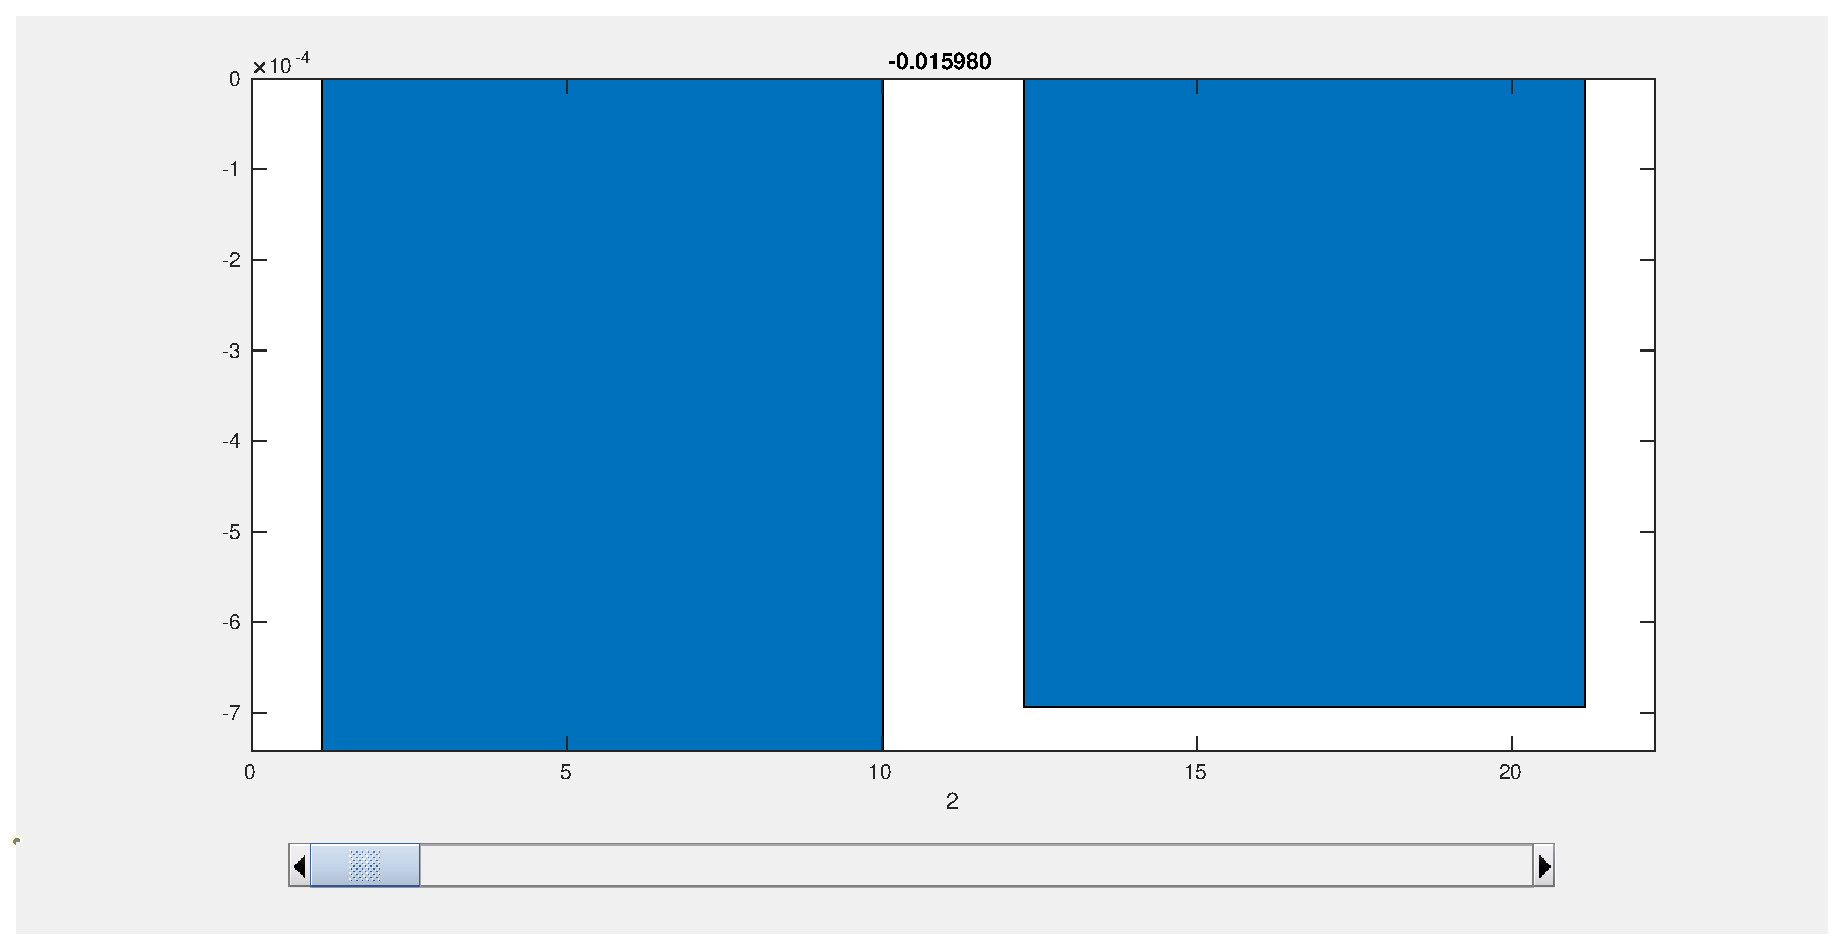
\includegraphics[scale=0.60, center]{eps/stepsOf10.eps}
    \caption{Step size of approximately 10}
    \label{fig:Riemann10}
\end{figure}
\begin{figure}[]
    \centering
    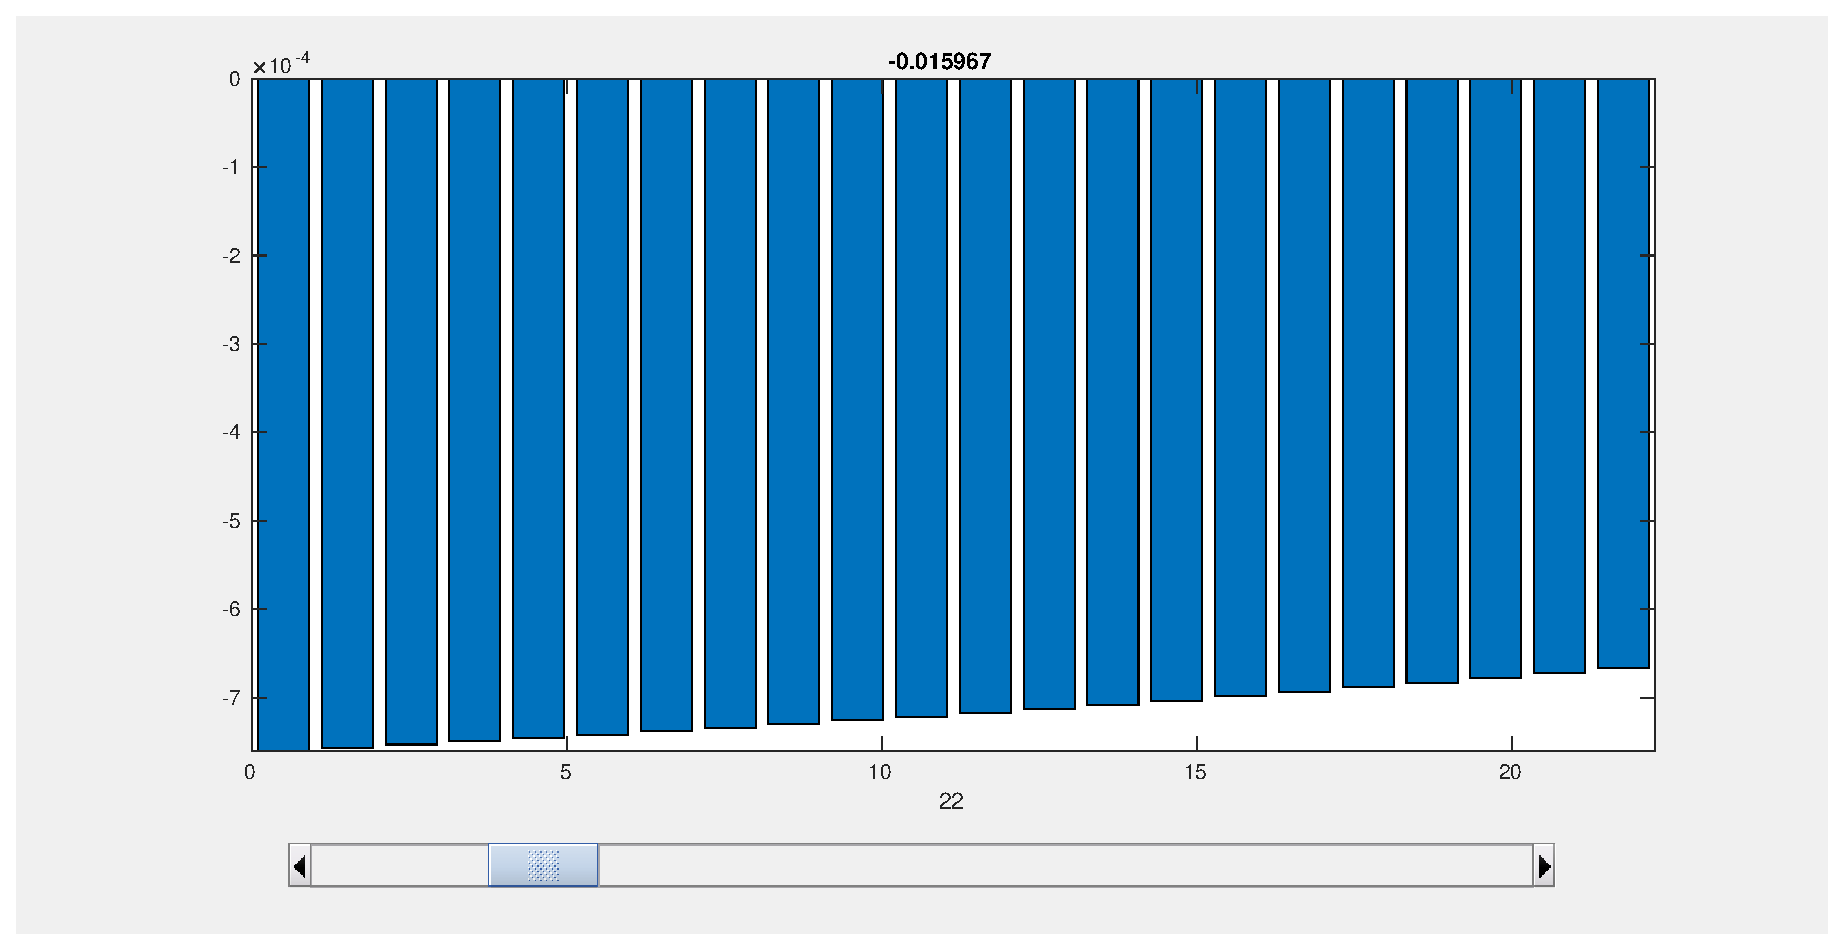
\includegraphics[scale=0.60, center]{eps/stepsOf1.eps}
    \caption{Step size of approximately 1}
    \label{fig:Riemann1}
\end{figure}